\subsection{Vorgehen}
\frame{
  \frametitle{Unsere ersten Versuche}
  
  \subsection{Google Eigenwert Matrix}
Potenzmethode\\

$$
\begin{bmatrix}
u_1 \\
u_2 \\
u_3 \\
u_4 \\
u_5 \\
u_6 \\
u_7 \\
u_8 \\
\end{bmatrix}
=
\begin{bmatrix}
\frac{1}{4} & \frac{1}{4} & 0 & 0 & 0 & 0 & 0 & 0 \\
\frac{1}{6} & \frac{1}{4} & \frac{1}{3} & 0 & 0 & 0 & 0 & 0 \\
0 & \frac{1}{2} & \frac{1}{3} & \frac{1}{2} & 0 & 0 & 0 & 0 \\
0 & 0 & \frac{1}{3} & \frac{1}{3} & \frac{1}{3} & 0 & 0 & 0 \\
0 & 0 & 0 & \frac{1}{5} & \frac{1}{3} & \frac{1}{5} & 0 & 0 \\
0 & 0 & 0 & 0 & \frac{1}{3} & \frac{1}{2} & \frac{1}{1} & 0 \\
0 & 0 & 0 & 0 & 0 & \frac{1}{3} & \frac{1}{3} & \frac{1}{5}\\
0 & 0 & 0 & 0 & 0 & 0 & \frac{1}{6} & \frac{1}{5} \\
\end{bmatrix}
\cdot
\begin{bmatrix}
1 \\
1 \\ 
1 \\
 1 \\
 1 \\
 1 \\ 
 1 \\
  1 \\
 
\end{bmatrix}
$$

%$
%\begin{bmatrix}
%0.4 & 0.6 & 0 & 0 & 0 & 0 & 0 & 0 & 0 & 0 & 0 & 0 & 0 & 0 & 0   \\
%0.2 & 0.3 & 0.5 & 0 & 0 & 0 & 0 & 0 & 0 & 0 & 0 & 0 & 0 & 0 & 0   \\
%0 & 0.4 & 0.4 & 0.2 & 0 & 0 & 0 & 0 & 0 & 0 & 0 & 0 & 0 & 0 & 0   \\
%0 & 0 & 0.1 & 0.7 & 0.2 & 0 & 0 & 0 & 0 & 0 & 0 & 0 & 0 & 0 & 0   \\
%0 & 0 & 0 & 0.3 & 0.3 & 0.4 & 0 & 0 & 0 & 0 & 0 & 0 & 0 & 0 & 0   \\
%0 & 0 & 0 & 0 & 0.3 & 0.6 & 0.1 & 0 & 0 & 0 & 0 & 0 & 0 & 0 & 0   \\
%0 & 0 & 0 & 0 & 0 & 0.1 & 0.1 & 0.8 & 0 & 0 & 0 & 0 & 0 & 0 & 0  \\
%0 & 0 & 0 & 0 & 0 & 0 & 0.6 & 0.3 & 0.1 & 0 & 0 & 0 & 0 & 0 & 0   \\
%0 & 0 & 0 & 0 & 0 & 0 & 0 & 0.2 & 0.4 & 0.4 & 0 & 0 & 0 & 0 & 0  \\
%0 & 0 & 0 & 0 & 0 & 0 & 0 & 0 & 0.3 & 0.2 & 0.5 & 0 & 0 & 0 & 0   \\
%0 & 0 & 0 & 0 & 0 & 0 & 0 & 0 & 0 & 0.2 & 0.2 & 0.6 & 0 & 0 & 0   \\
%0 & 0 & 0 & 0 & 0 & 0 & 0 & 0 & 0 & 0 & 0.5 & 0.3 & 0.2 & 0 & 0   \\
%0 & 0 & 0 & 0 & 0 & 0 & 0 & 0 & 0 & 0 & 0 & 0.7 & 0.2 & 0.1 & 0  \\
%0 & 0 & 0 & 0 & 0 & 0 & 0 & 0 & 0 & 0 & 0 & 0 & 0.5 & 0.2 & 0.3 \\
%0 & 0 & 0 & 0 & 0 & 0 & 0 & 0 & 0 & 0 & 0 & 0 & 0 & 0.2 & 0.2  \\
%
%\end{bmatrix}
%\qquad
%\begin{bmatrix}
%1 \\
%1 \\
%1 \\
%1 \\
%1 \\
%1 \\
%1 \\
%1 \\
%1 \\
%1 \\
%1 \\
%1 \\
%1 \\
%1 \\
%1 \\
%\end{bmatrix}
%
%\end{tiny}  


$$Eigenvektor=\dfrac{Eigenvektor \cdot Matrix}{Norm(Eigenvektor\cdot Matrix)}$$
$$Eigenwert\footnote{Betragsmässig grösster Eigenwert} = Eigenvektor \cdot Matrix \cdot Eigenvektor'$$
}

\frame
{

\begin{center}

\begin{tikzpicture}[scale = 0.7]
\draw[thick] (0,10) -- (0,-0.5);
\draw[thick] (0,10) -- (0.5,10);
\draw[thick] (0,-0.5) -- (0.5,-0.5);
\draw[thick] (10.5,10) -- (10.5,-0.5);
\draw[thick] (10.5,10) -- (10,10);
\draw[thick] (10,-0.5) -- (10.5,-0.5);
\draw[thick] (0.5,9.5) -- (0.5,6.5);
\draw[thick] (0.5,9.5) -- (1,9.5);
\draw[thick] (0.5,6.5) -- (1,6.5);
\draw[thick] (3.5,9.5) -- (3,9.5);
\draw[thick] (3.5,6.5) -- (3,6.5);
\draw[thick] (3.5,9.5) -- (3.5,6.5);
\draw[thick] (3.7,6.3) -- (3.7,3.3);
\draw[thick] (6.7,6.3) -- (6.7,3.3);
\draw[thick] (3.7,6.3) -- (4.2,6.3);
\draw[thick] (3.7,3.3) -- (4.2,3.3);
\draw[thick] (6.7,3.3) -- (6.2,3.3);
\draw[thick] (6.7,6.3) -- (6.2,6.3);
\draw[thick] (6.9,3) -- (6.9,0);
\draw[thick] (6.9,3) -- (7.4,3);
\draw[thick] (6.9,0) -- (7.4,0);
\draw[thick] (9.9,3) -- (9.9,0);
\draw[thick] (9.9,3) -- (9.4,3);
\draw[thick] (9.9,0) -- (9.4,0);

\draw[thick] (11.5,-0.5) -- (11.5,10);
\draw[thick] (11.5,-0.5) -- (12,-0.5);
\draw[thick] (11.5,10) -- (12,10);
\draw[thick] (14,-0.5) -- (14,10);
\draw[thick] (14,-0.5) -- (13.5,-0.5);
\draw[thick] (14,10) -- (13.5,10);

\draw[dashed] (3.5,9.5) -- (13.5,9.5);
\draw[dashed] (3.5,6.5) -- (13.5,6.5);
\draw[dashed] (6.7,6.3) -- (13.5,6.3);
\draw[dashed] (6.7,3.3) -- (13.5,3.3);
\draw[dashed] (9.7,3) -- (13.5,3);
\draw[dashed] (9.7,0) -- (13.5,0);
\end{tikzpicture}
\end{center}
}

\frame{
$$
\begin{bmatrix}
\frac{1}{4} & \frac{1}{4} & 0 & 0 & 0 & 0 & 0 & 0 & 0 & 0 & 0 & 0 \\
\frac{1}{6} & \frac{1}{4} & \frac{1}{3} & 0 & 0 & 0 & 0 & 0 & 0 & 0 & 0 & 0 \\
0 & \frac{1}{2} & \frac{1}{3} & \frac{1}{2} & 0 & 0 & 0 & 0 & 0 & 0 & 0 & 0 \\
0 & 0 & \frac{1}{3} & \frac{1}{4} & \frac{1}{2} & 0 & 0 & 0 & 0 & 0 & 0 & 0 \\
0 & 0 & 0 & \frac{1}{4} & \frac{1}{2} & \frac{1}{4} & 0 & 0 & 0 & 0 & 0 & 0 \\
0 & 0 & 0 & 0 & \frac{1}{6} & \frac{1}{4} & \frac{1}{3} & 0 & 0 & 0 & 0 & 0 \\
0 & 0 & 0 & 0 & 0 & \frac{1}{2} & \frac{1}{3} & \frac{1}{3} & 0 & 0 & 0 & 0 \\
0 & 0 & 0 & 0 & 0 & 0 & \frac{1}{3}  & \frac{1}{3} & \frac{1}{4} & 0 & 0 & 0 \\
0 & 0 & 0 & 0 & 0 & 0 & 0 & \frac{1}{4} & \frac{1}{4} & \frac{1}{4} & 0 & 0\\
0 & 0 & 0 & 0 & 0 & 0 & 0 & 0 & \frac{1}{2} & \frac{1}{4} & \frac{1}{3} & 0  \\
0 & 0 & 0 & 0 & 0 & 0 & 0 & 0 & 0 & \frac{1}{2} & \frac{1}{3} & \frac{1}{2}\\
0 & 0 & 0 & 0 & 0 & 0 & 0 & 0 &0 & 0 & \frac{1}{3} & \frac{1}{8} \\
\end{bmatrix}
$$

}

\frame{
$$
\begin{bmatrix}
\begin{bmatrix}
\frac{1}{4} & \frac{1}{4} & 0 & 0 \\
\frac{1}{6} & \frac{1}{4} & \frac{1}{3} & 0  \\
0 & \frac{1}{2} & \frac{1}{3} & \frac{1}{2} \\
0 & 0 & \frac{1}{3} & \frac{1}{4}  \\
\end{bmatrix}
\begin{bmatrix}
0 & 0 & 0 & 0 \\
0 & 0 & 0 & 0 \\
0 & 0 & 0 & 0 \\
\textcolor{red}{\frac{1}{2}} & 0 & 0 & 0 \\
\end{bmatrix}
\begin{bmatrix}
0 & 0 & 0 & 0 \\
0 & 0 & 0 & 0 \\
0 & 0 & 0 & 0 \\
0 & 0 & 0 & 0 \\
\end{bmatrix}
\\
\begin{bmatrix}
0 & 0 & 0 & \textcolor{red}{\frac{1}{4}} \\
0 & 0 & 0 & 0 \\
0 & 0 & 0 & 0 \\
0 & 0 & 0 & 0 \\
\end{bmatrix}
\begin{bmatrix}
\frac{1}{2} & \frac{1}{4} & 0 & 0 \\
\frac{1}{6} & \frac{1}{4} & \frac{1}{3} & 0  \\
0 & \frac{1}{2} & \frac{1}{3} & \frac{1}{3} \\
0 & 0 & \frac{1}{3} & \frac{1}{3}  \\
\end{bmatrix}
\begin{bmatrix}
0 & 0 & 0 & 0 \\
0 & 0 & 0 & 0 \\
0 & 0 & 0 & 0 \\
\textcolor{red}{\frac{1}{4}} & 0 & 0 & 0 \\
\end{bmatrix}
\\
\begin{bmatrix}
0 & 0 & 0 & 0 \\
0 & 0 & 0 & 0 \\
0 & 0 & 0 & 0 \\
0 & 0 & 0 & 0 \\
\end{bmatrix}
\begin{bmatrix}
0 & 0 & 0 & \textcolor{red}{\frac{1}{4}} \\
0 & 0 & 0 & 0 \\
0 & 0 & 0 & 0 \\
0 & 0 & 0 & 0 \\
\end{bmatrix}
\begin{bmatrix}
\frac{1}{4} & \frac{1}{4} & 0 & 0 \\
\frac{1}{2} & \frac{1}{4} & \frac{1}{3} & 0  \\
0 & \frac{1}{2} & \frac{1}{3} & \frac{1}{2} \\
0 & 0 & \frac{1}{3} & \frac{1}{8}  \\
\end{bmatrix}
\end{bmatrix}
$$

}

%\frame{
%$$
%\begin{bmatrix}
%\frac{1}{4} & \frac{1}{4} & 0 & 0 & 0 & 0 & 0 & 0 & 0 & 0 & 0 & 0 \\
%\frac{1}{6} & \frac{1}{4} & \frac{1}{3} & 0 & 0 & 0 & 0 & 0 & 0 & 0 & 0 & 0 \\
%0 & \frac{1}{2} & \frac{1}{3} & \frac{1}{2} & 0 & 0 & 0 & 0 & 0 & 0 & 0 & 0 \\
%0 & 0 & \frac{1}{3} & \frac{1}{4} & \textcolor{red}{\frac{1}{2}} & 0 & 0 & 0 & 0 & 0 & 0 & 0 \\
%0 & 0 & 0 & \textcolor{red}{\frac{1}{4}} & \frac{1}{2} & \frac{1}{4} & 0 & 0 & 0 & 0 & 0 & 0 \\
%0 & 0 & 0 & 0 & \frac{1}{6} & \frac{1}{4} & \frac{1}{3} & 0 & 0 & 0 & 0 & 0 \\
%0 & 0 & 0 & 0 & 0 & \frac{1}{2} & \frac{1}{3} & \frac{1}{3} & 0 & 0 & 0 & 0 \\
%0 & 0 & 0 & 0 & 0 & 0 & \frac{1}{3}  & \frac{1}{3} & \frac{1}{4} & 0 & 0 & 0 \\
%0 & 0 & 0 & 0 & 0 & 0 & 0 & \frac{1}{4} & \frac{1}{4} & \frac{1}{4} & 0 & 0\\
%0 & 0 & 0 & 0 & 0 & 0 & 0 & 0 & \frac{1}{2} & \frac{1}{4} & \frac{1}{3} & 0  \\
%0 & 0 & 0 & 0 & 0 & 0 & 0 & 0 & 0 & \frac{1}{2} & \frac{1}{3} & \frac{1}{2}\\
%0 & 0 & 0 & 0 & 0 & 0 & 0 & 0 &0 & 0 & \frac{1}{3} & \frac{1}{8} \\
%\end{bmatrix}
%$$
%
%}



\frame 
{
\begin{center}

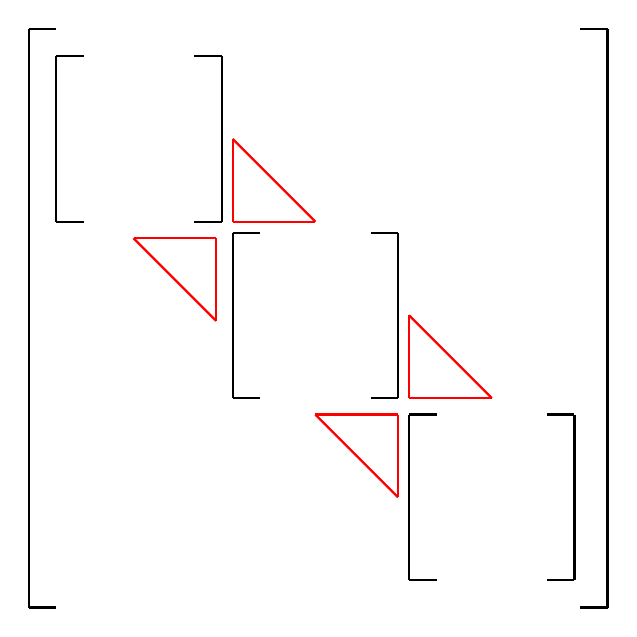
\begin{tikzpicture}[scale = 0.7]
\draw[thick] (0,10) -- (0,-0.5);
\draw[thick] (0,10) -- (0.5,10);
\draw[thick] (0,-0.5) -- (0.5,-0.5);
\draw[thick] (10.5,10) -- (10.5,-0.5);
\draw[thick] (10.5,10) -- (10,10);
\draw[thick] (10,-0.5) -- (10.5,-0.5);
\draw[thick] (0.5,9.5) -- (0.5,6.5);
\draw[thick] (0.5,9.5) -- (1,9.5);
\draw[thick] (0.5,6.5) -- (1,6.5);
\draw[thick] (3.5,9.5) -- (3,9.5);
\draw[thick] (3.5,6.5) -- (3,6.5);
\draw[thick] (3.5,9.5) -- (3.5,6.5);
\draw[thick] (3.7,6.3) -- (3.7,3.3);
\draw[thick] (6.7,6.3) -- (6.7,3.3);
\draw[thick] (3.7,6.3) -- (4.2,6.3);
\draw[thick] (3.7,3.3) -- (4.2,3.3);
\draw[thick] (6.7,3.3) -- (6.2,3.3);
\draw[thick] (6.7,6.3) -- (6.2,6.3);
\draw[thick] (6.9,3) -- (6.9,0);
\draw[thick] (6.9,3) -- (7.4,3);
\draw[thick] (6.9,0) -- (7.4,0);
\draw[thick] (9.9,3) -- (9.9,0);
\draw[thick] (9.9,3) -- (9.4,3);
\draw[thick] (9.9,0) -- (9.4,0);



\draw[thick,red] (3.7,6.5) -- (3.7,8);
\draw[thick,red] (3.7,6.5) -- (5.2,6.5);
\draw[thick,red] (3.7,8) -- (5.2,6.5);

\draw[thick,red] (6.9,3.3) -- (6.9,4.8);
\draw[thick,red] (6.9,3.3) -- (8.4,3.3);
\draw[thick,red] (6.9,4.8) -- (8.4,3.3);

\draw[thick,red] (6.7,3) -- (6.7,1.5);
\draw[thick,red] (6.7,3) -- (5.2,3);
\draw[thick,red] (5.2,3) -- (6.7,1.5);

\draw[thick,red] (3.4,6.2) -- (3.4,4.7);
\draw[thick,red] (3.4,6.2) -- (1.9,6.2);
\draw[thick,red] (1.9,6.2) -- (3.4,4.7);

\end{tikzpicture}
\end{center}
}
\frame{
\begin{center}
\begin{tikzpicture}[scale = 0.7]
\draw[thick] (0,10) -- (0,-0.5);
\draw[thick] (0,10) -- (0.5,10);
\draw[thick] (0,-0.5) -- (0.5,-0.5);
\draw[thick] (10.5,10) -- (10.5,-0.5);
\draw[thick] (10.5,10) -- (10,10);
\draw[thick] (10,-0.5) -- (10.5,-0.5);
\draw[thick] (0.5,9.5) -- (0.5,6.5);
\draw[thick] (0.5,9.5) -- (1,9.5);
\draw[thick] (0.5,6.5) -- (1,6.5);
\draw[thick] (3.5,9.5) -- (3,9.5);
\draw[thick] (3.5,6.5) -- (3,6.5);
\draw[thick] (3.5,9.5) -- (3.5,6.5);
\draw[thick] (3.7,6.3) -- (3.7,3.3);
\draw[thick] (6.7,6.3) -- (6.7,3.3);
\draw[thick] (3.7,6.3) -- (4.2,6.3);
\draw[thick] (3.7,3.3) -- (4.2,3.3);
\draw[thick] (6.7,3.3) -- (6.2,3.3);
\draw[thick] (6.7,6.3) -- (6.2,6.3);
\draw[thick] (6.9,3) -- (6.9,0);
\draw[thick] (6.9,3) -- (7.4,3);
\draw[thick] (6.9,0) -- (7.4,0);
\draw[thick] (9.9,3) -- (9.9,0);
\draw[thick] (9.9,3) -- (9.4,3);
\draw[thick] (9.9,0) -- (9.4,0);

\draw[dashed] (2,8.2) -- (2,5.2);
\draw[dashed] (2,8.2) -- (2.5,8.2);
\draw[dashed] (2,5.2) -- (2.5,5.2);
\draw[dashed] (5,8.2) -- (5,5.2);
\draw[dashed] (5,5.2) -- (4.5,5.2);
\draw[dashed] (5,8.2) -- (4.5,8.2);

\draw[dashed] (5.2,4.9) -- (5.2,1.9);
\draw[dashed] (5.2,4.9) -- (5.7,4.9);
\draw[dashed] (5.2,1.9) -- (5.7,1.9);
\draw[dashed] (8.2,4.9) -- (8.2,1.9);
\draw[dashed] (8.2,4.9) -- (7.7,4.9);
\draw[dashed] (8.2,1.9) -- (7.7,1.9);


\draw[thick] (11.5,-0.5) -- (11.5,10);
\draw[thick] (11.5,-0.5) -- (12,-0.5);
\draw[thick] (11.5,10) -- (12,10);
\draw[thick] (14,-0.5) -- (14,10);
\draw[thick] (14,-0.5) -- (13.5,-0.5);
\draw[thick] (14,10) -- (13.5,10);
\end{tikzpicture}
\end{center}
}
\frame
{
\frametitle{Erste Veruche mit Matlab}

\begin{center}
Erstellte dünnbesetzte Bandmatrix mit Matlab
\\

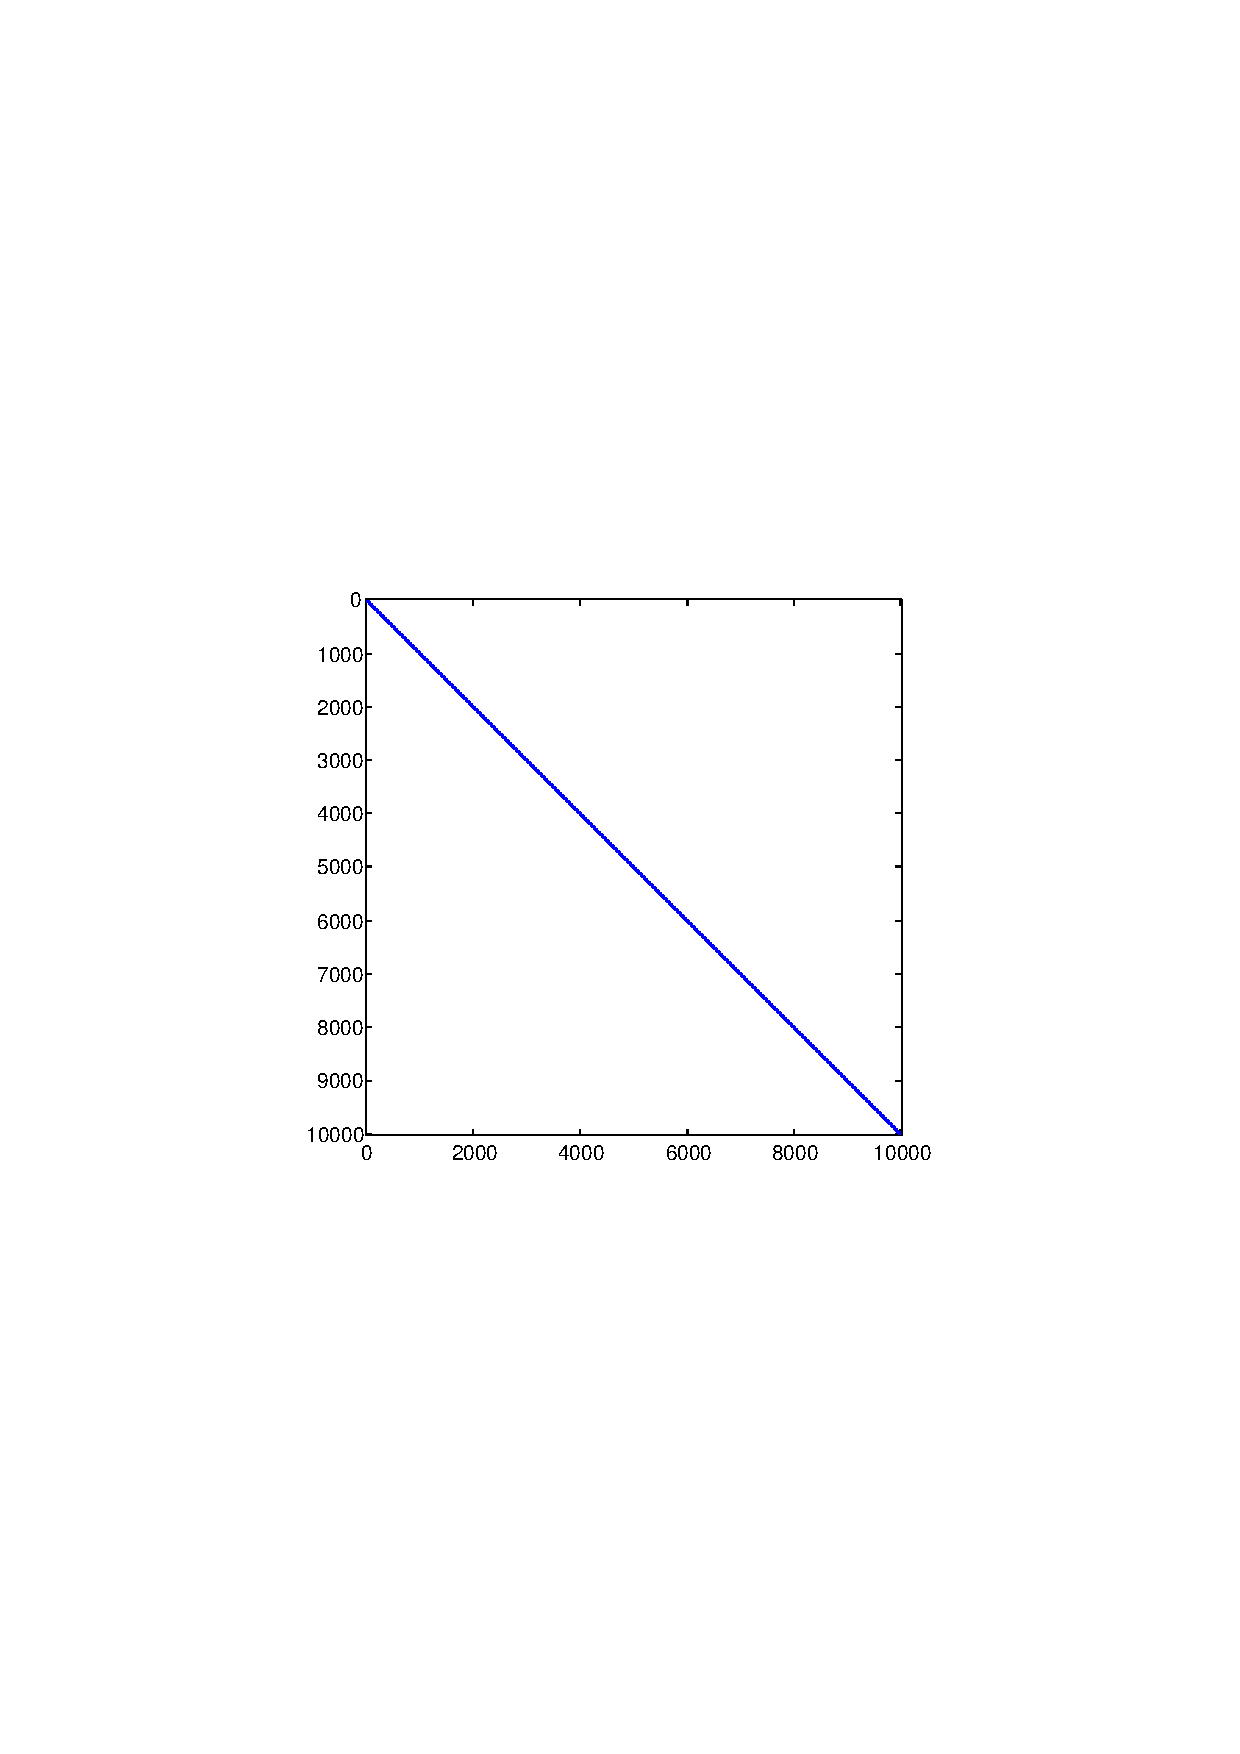
\includegraphics[width=0.5\textwidth]{./Bilder/spy}
\end{center}
}
\frame
{
\lstinputlisting[breaklines=true]{es.m}
}



%%% Local Variables: 
%%% mode: latex
%%% TeX-master: "main"
%%% End: 
